\documentclass[10pt, aspectratio=169, handout]{beamer}
\usefonttheme{professionalfonts}

\mode<presentation>
{
  \usetheme{Berkeley}
  \usecolortheme{beaver}
  \usefonttheme{default}
  \setbeamertemplate{navigation symbols}{}
  \setbeamertemplate{caption}[numbered]
} 

\setbeamertemplate{footline}{%
  \leavevmode%
  \hbox{%
    \begin{beamercolorbox}[wd=.85\paperwidth,ht=2.5ex,dp=1ex,left]{author in head/foot}%
      \usebeamerfont{author in head/foot}Maxx Seminario, Electronic Circuits, Spring 2026%
    \end{beamercolorbox}%
    \begin{beamercolorbox}[wd=.15\paperwidth,ht=2.5ex,dp=1ex,right]{date in head/foot}%
      \hspace*{0.5em}\insertframenumber{} / \inserttotalframenumber\hspace*{0.5em}%
    \end{beamercolorbox}%
  }%
  \vskip0pt%
}

\usepackage[english]{babel}
\usepackage[utf8]{inputenc}
\usepackage{tikz}
\usepackage{pgfplots}
\usepackage{array}
\usepackage{makecell}
\usepackage{verbatim}
\usepackage{graphicx}
\usepackage{subcaption}
\usepackage{amsfonts}
\usepackage{amsmath}
\usepackage{bm}
\usepackage{epstopdf}
\usepackage[american]{circuitikz}
\usepackage{caption}
\captionsetup{compatibility=false}
\usepackage[absolute,overlay]{textpos}
\usetikzlibrary{calc}
\usetikzlibrary{pgfplots.fillbetween, backgrounds}
\usetikzlibrary{positioning}
\usetikzlibrary{pgfplots.groupplots}
\usetikzlibrary{plotmarks}
\usetikzlibrary{calc}
\usetikzlibrary{decorations.markings}
\usetikzlibrary{arrows.meta,calc}

\usepgfplotslibrary{groupplots}
\pgfplotsset{compat=newest} 

\usepackage{hyperref}
\hypersetup{
    colorlinks=true,
    linkcolor=blue,
    filecolor=magenta,      
    urlcolor=cyan,
}

% Added by Maxx Seminario 01/06/2026 - for colored icons in itemize labels
\usepackage{wasysym} % for smiles and frowns
\newcommand{\neutralface}{%
  \tikz[baseline=-0.6ex]{
    \draw (0,0) circle (0.9ex);
    \fill (-0.35ex,0.25ex) circle (0.12ex);
    \fill ( 0.35ex,0.25ex) circle (0.12ex);
    \draw (-0.35ex,-0.25ex) -- (0.35ex,-0.25ex);
  }%
}
\newcommand{\baditem}{\textcolor{red!70!black}{\frownie}}
\newcommand{\gooditem}{\textcolor{green!60!black}{\smiley}}
\newcommand{\mehitem}{\textcolor{orange!80!black}{\neutralface}}

\title[ECEN 222]{Diode Applications: Rectifiers and Power Supplies}
\author{Maxx Seminario}
\institute{University of Nebraska-Lincoln}
\date{Spring 2026}

\begin{document}
\begin{frame}
  \titlepage
\end{frame}

\section{Introduction}

\begin{frame}{Diode Applications Overview}
    
    \begin{columns}[t]
    \column{0.48\textwidth}
        \textbf{Why Study Rectifiers?}:
        \begin{itemize}
            \item Most electronics need DC power
            \item Wall outlets provide AC power
            \item Rectifiers convert AC to DC
            \item Foundation of power supplies
        \end{itemize}
        
        \vspace{0.5em}
        \textbf{Key Applications}:
        \begin{itemize}
            \item Battery chargers
            \item Computer power supplies
            \item LED drivers
            \item Motor controllers
        \end{itemize}
    
    \column{0.48\textwidth}
        \textbf{Topics We'll Cover}:
        \begin{itemize}
            \item Half-wave rectifiers
            \item Full-wave rectifiers
            \item Bridge rectifiers
            \item Filtering capacitors
            \item Ripple voltage
            \item Voltage regulation with Zeners
        \end{itemize}
        
        \vspace{0.5em}
        \begin{center}
        \begin{circuitikz}[scale=0.8]
            \draw (0,0) to[sV, l=$v_{AC}$] (0,2)
                to[D] (2,2)
                to[R, l=$R_L$] (2,0)
                to[short] (0,0);
            \draw (3,1) node[right] {Simple Rectifier};
        \end{circuitikz}
        \end{center}
    
    \end{columns}
    
\end{frame}

\section{Half-Wave Rectifiers}

\begin{frame}{Half-Wave Rectifier Circuit}
    
    \begin{columns}[t]
    \column{0.48\textwidth}
        \textbf{Basic Circuit}:
        
        \begin{center}
        \begin{circuitikz}[american, scale=0.8]
            \draw (0,0) to[sV, l=$v_{AC}$] (0,3)
                  to[D, l=$D$] (3,3)
                  to[R, l=$R_L$, v=$v_o$] (3,0)
                  to[short] (0,0);
            \draw (1.5,0) node[ground]{};
        \end{circuitikz}
        \end{center}
        
        \vspace{-0.5cm}

        \textbf{Operation}:
        \begin{itemize}
            \item Input: $v_{AC} = V_p \sin(\omega t)$
            \item Positive half-cycle: diode ON
            \item Negative half-cycle: diode OFF
            \item Output: positive half-waves only
        \end{itemize}
        
    \column{0.48\textwidth}
        \textbf{Waveforms}:
        
        \begin{center}
        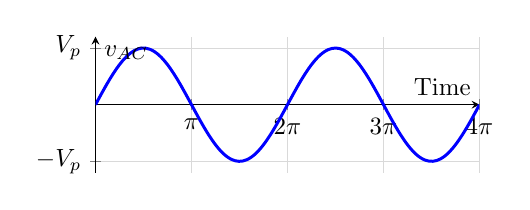
\begin{tikzpicture}[scale=0.9]
            \begin{axis}[
                width=7cm, 
                height=3.5cm,
                xlabel={Time},
                ylabel={$v_{AC}$},
                xmin=0, 
                xmax=4*pi,
                ymin=-1.2, 
                ymax=1.2,
                grid=major,
                grid style={line width=0.1pt, draw=gray!30},
                axis lines=middle,
                xtick={0, pi, 2*pi, 3*pi, 4*pi},
                xticklabels={0, $\pi$, $2\pi$, $3\pi$, $4\pi$},
                ytick={-1,0,1},
                yticklabels={$-V_p$,0,$V_p$},
            ]
            \addplot[blue, very thick, smooth, domain=0:4*pi, samples=100] {sin(deg(x))};
            \end{axis}
        \end{tikzpicture}
        
        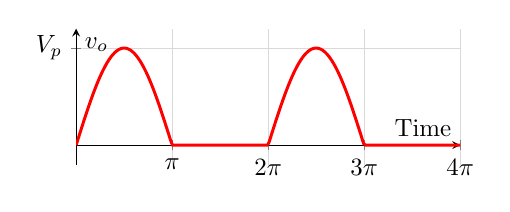
\begin{tikzpicture}[scale=0.9]
            \begin{axis}[
                width=7cm, 
                height=3.5cm,
                xlabel={Time},
                ylabel={$v_o$},
                xmin=0, 
                xmax=4*pi,
                ymin=-0.2, 
                ymax=1.2,
                grid=major,
                grid style={line width=0.1pt, draw=gray!30},
                axis lines=middle,
                xtick={0, pi, 2*pi, 3*pi, 4*pi},
                xticklabels={0, $\pi$, $2\pi$, $3\pi$, $4\pi$},
                ytick={0,1},
                yticklabels={0,$V_p$},
            ]
            \addplot[red, very thick, smooth, domain=0:4*pi, samples=200] {max(sin(deg(x)),0)};
            \end{axis}
        \end{tikzpicture}
        \end{center}
        
    \end{columns}
    
\end{frame}

\begin{frame}{Half-Wave Rectifier Analysis}
    
    \begin{columns}[t]
    \column{0.48\textwidth}
        \textbf{Average (DC) Output Voltage}:
        
        For ideal diode ($V_D = 0$):
        \begin{equation*}
            V_{DC} = \frac{V_p}{\pi} \approx 0.318 V_p
        \end{equation*}
        
        For real silicon diode ($V_D \approx 0.7$ V):
        \begin{equation*}
            V_{DC} = \frac{V_p - V_D}{\pi}
        \end{equation*}
        
        \vspace{0.5em}
        \textbf{Peak Inverse Voltage (PIV)}:
        \begin{itemize}
            \item Maximum reverse voltage on diode
            \item PIV $= V_p$
            \item Must select diode with PIV $> V_p$
        \end{itemize}
        
    \column{0.48\textwidth}
        \textbf{Example Calculation}:
        
        Given: $V_{AC,RMS} = 12$ V
        
        \begin{enumerate}
            \item Peak voltage: \\
            $V_p = \sqrt{2} \times V_{RMS} = 16.97$ V
            
            \item Calculate DC output: \\
            $V_{DC} = \frac{16.97 - 0.7}{\pi} = \frac{16.27}{\pi} = 5.18$ V
            
            \item PIV requirement: \\
            PIV $\geq 16.97$ V
        \end{enumerate}
        
        \vspace{0.5em}
        \textbf{Limitations}:
        \begin{itemize}
            \item[\baditem] Low DC output (only 31.8\%)
            \item[\baditem] Poor power utilization
            \item[\baditem] Large ripple voltage
        \end{itemize}
        
    \end{columns}
    
\end{frame}

\begin{frame}{Half-Wave Rectifier with Filter Capacitor}
    
    \begin{columns}[t]
    \column{0.48\textwidth}
        \textbf{Filtered Rectifier}:
        
        \begin{center}
        \begin{circuitikz}[american, scale=0.8]
            \draw (0,0) to[sV, l=$v_{AC}$] (0,3)
                  to[D, l=$D$] (3,3)
                  to[short] (4.5,3);
            \draw (3,3) to[R, l=$R_L$, v=$v_o$] (3,0);
            \draw (4.5,3) to[C, l=$C$] (4.5,0);
            \draw (0,0) to[short] (4.5,0);
            \draw (2.25,0) node[ground]{};
        \end{circuitikz}
        \end{center}
        
        \vspace{-0.5cm}

        \textbf{Operation}:
        \begin{itemize}
            \item Capacitor charges to $\approx V_p$ 
            \item Capacitor discharges through $R_L$ 
            \item Creates "ripple" voltage
            \item DC voltage higher than unfiltered
        \end{itemize}
        
    \column{0.48\textwidth}
        \textbf{Output Waveform}:
        
        \begin{center}
        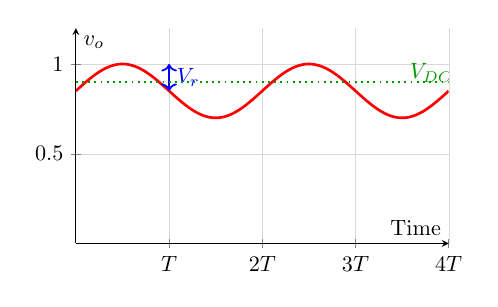
\begin{tikzpicture}[scale=0.8]
            \begin{axis}[
                width=7.5cm, 
                height=5cm,
                xlabel={Time},
                ylabel={$v_o$},
                xmin=0, 
                xmax=4*pi,
                ymin=0, 
                ymax=1.2,
                grid=major,
                grid style={line width=0.1pt, draw=gray!30},
                axis lines=middle,
                xtick={0, pi, 2*pi, 3*pi, 4*pi},
                xticklabels={0, $T$, $2T$, $3T$, $4T$},
            ]
            
            % Draw envelope
            \addplot[red, very thick, domain=0:4*pi, samples=200] 
                {max(0.85 + 0.15*sin(deg(x)), sin(deg(x)))};
            
            % Annotate ripple
            \draw[<->, blue, thick] (axis cs:pi,0.85) -- (axis cs:pi,1.0);
            \node[blue, right] at (axis cs:pi,0.925) {$V_r$};
            
            % Draw DC level line
            \draw[green!60!black, thick, dotted] (axis cs:0,0.9) -- (axis cs:4*pi,0.9);
            \node[green!60!black, right] at (axis cs:3.5*pi,0.95) {$V_{DC}$};
            
            \end{axis}
        \end{tikzpicture}
        \end{center}
        
        \vspace{-0.3cm}
        \textbf{Ripple Voltage}:
        \begin{equation*}
            V_r \approx \frac{V_p}{f R_L C}
        \end{equation*}
        
    \end{columns}
    
\end{frame}

\begin{frame}{Ripple Voltage Analysis}
    
    \begin{columns}[t]
    \column{0.48\textwidth}
        \textbf{Key Equations}:
        
        Ripple voltage (peak-to-peak):
        \begin{equation*}
            V_r \approx \frac{V_p}{f R_L C}
        \end{equation*}

        \vspace{-0.4cm}
        
        DC output voltage:
        \begin{equation*}
            V_{DC} \approx V_p - \frac{V_r}{2}
        \end{equation*}

        \vspace{-0.5cm}
        
        Ripple factor:
        \begin{equation*}
            r = \frac{V_{r,RMS}}{V_{DC}}
        \end{equation*}

        \vspace{-0.3cm}

        \textbf{Design Guidelines}:
        \begin{itemize}
            \item[\gooditem] Larger $C$ reduces ripple
            \item[\gooditem] Larger $R_L$ reduces ripple
            \item[\gooditem] Higher frequency reduces ripple
        \end{itemize}
        
    \column{0.48\textwidth}
        \textbf{Example}:
        
        Given: 
        \begin{itemize}
            \item $V_p = 17$ V
            \item $f = 60$ Hz
            \item $R_L = 2.2$ k$\Omega$
            \item $C = 470$ $\mu$F
        \end{itemize}
        
        Calculate ripple:
        \begin{align*}
            V_r &= \frac{17}{60 \times 2200 \times 470 \times 10^{-6}} = 0.274 \text{ V}
        \end{align*}

        \vspace{-0.2cm}

        \begin{equation*}
            V_{DC} = 17 - \frac{0.274}{2} = 16.86 \text{ V}
        \end{equation*}
        
        \vspace{-0.3cm}
        \textbf{Trade-offs}:
        \begin{itemize}
            \item Large $C$: less ripple, larger size
            \item Peak diode current increases with $C$
        \end{itemize}
        
    \end{columns}
    
\end{frame}

\section{Full-Wave Rectifiers}

\begin{frame}{Bridge Rectifier Circuit}
    
    \begin{columns}[t]
    \column{0.48\textwidth}
        \textbf{Bridge Configuration}:
        
        \begin{center}
        \begin{circuitikz}[american, scale=0.8]
            % AC source on left
            \draw (-2,0) to[sV, l=$v_{AC}$] (0,0);
            
            % Bridge diodes in diamond configuration
            % Left to top (D1)
            \draw (0,0) to[D, l=$D_1$, *-] (1.5,1.5);
            % Left to bottom (D2)
            \draw (0,0) to[D, l_=$D_2$, invert] (1.5,-1.5);
            % Top to right (D3)
            \draw (1.5,1.5) to[D, l=$D_3$, -*, invert] (3,0);
            % Bottom to right (D4)  
            \draw (1.5,-1.5) to[D, l_=$D_4$] (3,0);
            
            % Load between top and bottom
            \draw (1.5,1.5) to[short, *-] (4.5,1.5)
                  to[R, l=$R_L$, v=$v_o$] (4.5,-1.5)
                  to[short, -*] (1.5,-1.5);
            
            % Ground symbols
            % \draw (1.5,-1.5) node[ground]{};
            \draw (-2,0) node[ground]{};
            \draw (3,0) node[ground]{};
        \end{circuitikz}
        \end{center}
        
        \vspace{-0.8cm}
        \textbf{Operation}:
        \begin{itemize}
            \item Positive half-cycle: $D_1$, $D_4$ conduct
            \item Negative half-cycle: $D_2$, $D_3$ conduct
            \item Both half-cycles produce output
            \item Two diodes always in series
        \end{itemize}
        
    \column{0.48\textwidth}
        \textbf{Output Characteristics}:
        \begin{itemize}
            \item $v_o$ is always positive
            \item Output is full-wave rectified
            \item Continuous current through load
        \end{itemize}
        
        \vspace{0.5em}
        \textbf{Advantages}:
        \begin{itemize}
            \item[\gooditem] No center-tap transformer needed
            \item[\gooditem] Full-wave rectification
            \item[\gooditem] Higher DC output
            \item[\gooditem] Lower ripple frequency (2$f$)
        \end{itemize}
        
        \textbf{Disadvantages}:
        \begin{itemize}
            \item[\baditem] Two diode drops ($\approx 1.4$ V)
            \item[\baditem] Requires four diodes
        \end{itemize}
        
    \end{columns}

\end{frame}

\begin{frame}{Bridge Rectifier Analysis}
    
    \begin{columns}[t]
    \column{0.48\textwidth}
        \textbf{DC Output Voltage}:
        
        For ideal diodes ($V_D = 0$):
        \begin{equation*}
            V_{DC} = \frac{2V_p}{\pi} \approx 0.637 V_p
        \end{equation*}
        
        For real silicon diodes ($V_D \approx 0.7$ V each):
        \begin{equation*}
            V_{DC} = \frac{2(V_p - 2V_D)}{\pi}
        \end{equation*}
        
        \vspace{0.5em}
        \textbf{Peak Inverse Voltage}:
        \begin{itemize}
            \item Each diode: PIV $= V_p$
            \item Lower than center-tap configuration
        \end{itemize}
        
        \vspace{0.5em}
        \textbf{Comparison to Half-Wave}:
        \begin{itemize}
            \item DC output is 2x higher
            \item Ripple frequency is 2x higher
            \item Better power utilization
        \end{itemize}
        
    \column{0.48\textwidth}
        \textbf{Output Waveform}:
        
        \begin{center}
        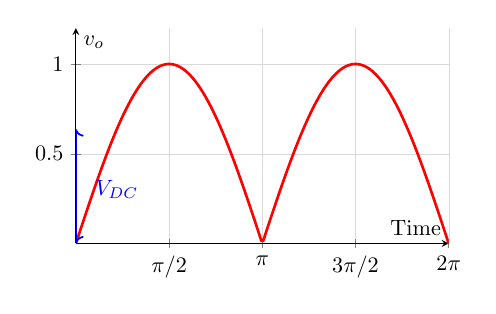
\begin{tikzpicture}[scale=0.8]
            \begin{axis}[
                width=7.5cm, 
                height=5cm,
                xlabel={Time},
                ylabel={$v_o$},
                xmin=0, 
                xmax=2*pi,
                ymin=0, 
                ymax=1.2,
                grid=major,
                grid style={line width=0.1pt, draw=gray!30},
                axis lines=middle,
                xtick={0, pi/2, pi, 3*pi/2, 2*pi},
                xticklabels={0, $\pi/2$, $\pi$, $3\pi/2$, $2\pi$},
            ]
            \addplot[red, very thick, smooth, domain=0:2*pi, samples=200] {abs(sin(deg(x)))};
            
            \draw[<->, blue, thick] (axis cs:0,0) -- (axis cs:0,0.637);
            \node[blue, right] at (axis cs:0.2,0.3) {$V_{DC}$};
            \end{axis}
        \end{tikzpicture}
        \end{center}
        
        \vspace{-0.3cm}
        \textbf{Example}:
        
        $V_{AC,RMS} = 12$ V, $V_p = 16.97$ V
        
        \begin{equation*}
            V_{DC} = \frac{2(16.97 - 1.4)}{\pi} = \frac{31.14}{\pi} = 9.91 \text{ V}
        \end{equation*}
        
        Compare to half-wave: 5.18 V (nearly 2x improvement!)
        
    \end{columns}
    
\end{frame}

\begin{frame}{Bridge Rectifier with Filter}
    
    \begin{columns}[t]
    \column{0.48\textwidth}
        \textbf{Filtered Bridge Rectifier}:
        
        \begin{center}
        \begin{circuitikz}[american, scale=0.8]
            % AC source
            \draw (0,2) to[sV, l=$v_{AC}$] (0,0);
            
            % Bridge
            \draw (0,2) to[short] (1,3)
                  to[D, l=$D_1$] (3,3)
                  to[short] (4,2);
            \draw (0,0) to[short] (1,-1)
                  to[D, l_=$D_3$] (3,-1)
                  to[short] (4,0);
            \draw (1,3) to[D, l=$D_2$, *-*] (1,-1);
            \draw (3,3) to[D, l_=$D_4$, *-*] (3,-1);
            
            % Load and filter
            \draw (4,2) to[short] (5.5,2);
            \draw (4,2) to[R, l=$R_L$] (4,0);
            \draw (5.5,2) to[C, l=$C$] (5.5,0);
            \draw (4,0) to[short] (5.5,0);
            \draw (2.75,0.5) node[ground]{};
        \end{circuitikz}
        \end{center}
        
        \vspace{0.5em}
        \textbf{Key Difference}:
        
        Ripple frequency is \textbf{2$f$} (120 Hz for 60 Hz AC)
        
        \begin{equation*}
            V_r \approx \frac{V_p}{2f R_L C}
        \end{equation*}
        
        Ripple is \textbf{half} that of half-wave rectifier with same $C$!
        
    \column{0.48\textwidth}
        \textbf{Output Waveform}:
        
        \begin{center}
        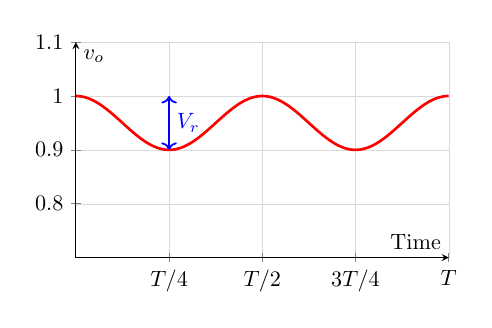
\begin{tikzpicture}[scale=0.8]
            \begin{axis}[
                width=7.5cm, 
                height=5cm,
                xlabel={Time},
                ylabel={$v_o$},
                xmin=0, 
                xmax=2*pi,
                ymin=0.7, 
                ymax=1.1,
                grid=major,
                grid style={line width=0.1pt, draw=gray!30},
                axis lines=middle,
                xtick={0, pi/2, pi, 3*pi/2, 2*pi},
                xticklabels={0, $T/4$, $T/2$, $3T/4$, $T$},
            ]
            
            % Approximation of filtered output
            \addplot[red, very thick, domain=0:2*pi, samples=400] 
                {0.95 + 0.05*cos(2*deg(x))};
            
            \draw[<->, blue, thick] (axis cs:pi/2,0.9) -- (axis cs:pi/2,1.0);
            \node[blue, right] at (axis cs:pi/2,0.95) {$V_r$};
            
            \end{axis}
        \end{tikzpicture}
        \end{center}
        
        \vspace{-0.3cm}
        \textbf{Design Example}:
        
        Same parameters as before, but $f$ → $2f$:
        
        \begin{align*}
            V_r &= \frac{17}{2 \times 60 \times 2200 \times 470 \times 10^{-6}} \\
            &= \frac{17}{124.08} = 0.137 \text{ V}
        \end{align*}
        
        Only \textbf{half} the ripple of half-wave!
        
    \end{columns}
    
\end{frame}

\section{Voltage Regulation}

\begin{frame}{Need for Voltage Regulation}
    
    \begin{columns}[t]
    \column{0.48\textwidth}
        \textbf{The Problem}:
        
        \begin{itemize}
            \item Rectifier output varies with:
            \begin{itemize}
                \item Input (line) voltage changes
                \item Load current changes
                \item Ripple voltage
            \end{itemize}
            \item Most circuits need stable DC
            \item Example: Logic circuits need ±5\% tolerance
        \end{itemize}
        
        \vspace{0.5em}
        \textbf{The Solution}:
        
        Voltage regulator:
        \begin{itemize}
            \item Maintains constant output voltage
            \item Compensates for input variations
            \item Compensates for load variations
            \item Types: Linear, switching, Zener
        \end{itemize}
        
    \column{0.48\textwidth}
        \textbf{Block Diagram}:
        
        \begin{center}
        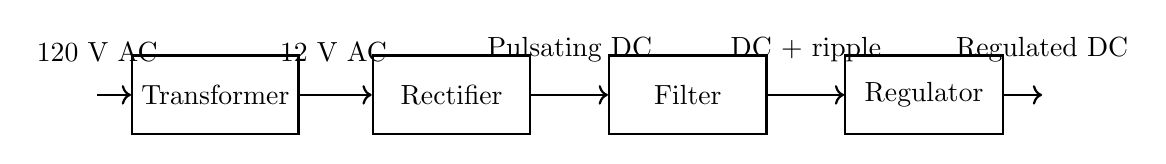
\begin{tikzpicture}[
            block/.style={rectangle, draw, thick, minimum width=2cm, minimum height=1cm}
        ]
            \node[block] (trans) at (0,0) {Transformer};
            \node[block] (rect) at (3,0) {Rectifier};
            \node[block] (filt) at (6,0) {Filter};
            \node[block] (reg) at (9,0) {Regulator};
            
            \draw[->, thick] (-1.5,0) -- (trans);
            \draw[->, thick] (trans) -- (rect);
            \draw[->, thick] (rect) -- (filt);
            \draw[->, thick] (filt) -- (reg);
            \draw[->, thick] (reg) -- (10.5,0);
            
            \node[above] at (-1.5,0.3) {120 V AC};
            \node[above] at (1.5,0.3) {12 V AC};
            \node[above] at (4.5,0.3) {Pulsating DC};
            \node[above] at (7.5,0.3) {DC + ripple};
            \node[above] at (10.5,0.3) {Regulated DC};
        \end{tikzpicture}
        \end{center}
        
        \vspace{0.5em}
        \textbf{Performance Metrics}:
        \begin{itemize}
            \item \textbf{Load regulation}: how much $V_o$ changes with load
            \item \textbf{Line regulation}: how much $V_o$ changes with input
            \item \textbf{Efficiency}: $P_{out}/P_{in}$
        \end{itemize}
        
    \end{columns}
    
\end{frame}

\begin{frame}{Zener Diode Shunt Regulator}
    
    \begin{columns}[t]
    \column{0.48\textwidth}
        \textbf{Basic Shunt Regulator}:
        
        \begin{center}
        \begin{circuitikz}[american, scale=1.1]
            \draw (0,3) to[V, l=$V_{in}$] (0,0);
            \draw (0,3) to[R, l=$R_S$, i>^=$I_S$] (3,3);
            
            % Zener branch 
            \draw (3,3) to[short] (4.0,3)
                  to[zD, l_=$D_Z$, v^=$V_Z$, i>_=$I_Z$] (4.0,0);
            
            % Load branch 
            \draw (3,3) to[short] (6,3)
                  to[R, l_=$R_L$, v^=$V_o$, i>_=$I_L$] (6,0);
            
            % Return
            \draw (0,0) to[short] (6,0);
            \draw (3,0) node[ground]{};
        \end{circuitikz}
        \end{center}
        
        \vspace{0.5em}
        \textbf{Operation Principle}:
        \begin{itemize}
            \item Zener maintains constant $V_Z$
            \item $R_S$ drops excess voltage
            \item Zener absorbs current variations
            \item $I_S = I_Z + I_L$ (KCL)
        \end{itemize}
        
    \column{0.48\textwidth}
        \textbf{Key Equations}:
        
        Series resistor current:
        \begin{equation*}
            I_S = \frac{V_{in} - V_Z}{R_S}
        \end{equation*}
        
        Kirchhoff's current law:
        \begin{equation*}
            I_Z = I_S - I_L
        \end{equation*}
        
        Zener power dissipation:
        \begin{equation*}
            P_Z = V_Z \cdot I_Z
        \end{equation*}
        
        \vspace{0.5em}
        \textbf{Design Constraints}:
        \begin{itemize}
            \item $I_Z \geq I_{Z,min}$ (stay in breakdown)
            \item $P_Z \leq P_{Z,max}$ (power rating)
            \item Worst case: max $I_L$, min $V_{in}$
            \item Best efficiency at full load
        \end{itemize}
        
    \end{columns}
    
\end{frame}

\begin{frame}{Shunt Regulator Design Example}
    
    \begin{columns}[t]
    \column{0.48\textwidth}
        \textbf{Design Specifications}:
        
        \begin{itemize}
            \item Output: $V_o = 5.1$ V (use 5.1 V Zener)
            \item Input: $V_{in} = 12$ V (from filtered rectifier)
            \item Load: $I_L = 0$ to 50 mA
            \item Zener: $I_{Z,min} = 5$ mA, $P_{Z,max} = 500$ mW
        \end{itemize}
        
        \vspace{0.5em}
        \textbf{Design Process}:
        
        \textbf{Step 1}: Choose $I_S$ at no-load
        
        Let $I_S = 2 \times I_{L,max} = 100$ mA
        
        This ensures enough current for regulation
        
        \vspace{0.5em}
        \textbf{Step 2}: Calculate $R_S$
        
        \begin{equation*}
            R_S = \frac{V_{in} - V_Z}{I_S} = \frac{12 - 5.1}{0.1} = 69 \text{ }\Omega
        \end{equation*}
        
        Use standard value: $R_S = 68$ $\Omega$
        
    \column{0.48\textwidth}
        \textbf{Step 3}: Verify worst-case conditions
        
        At no load ($I_L = 0$):
        \begin{align*}
            I_Z &= I_S - I_L = 100 - 0 = 100 \text{ mA} \\
            P_Z &= 5.1 \times 0.1 = 510 \text{ mW}
        \end{align*}
        
        \textbf{Problem!} Exceeds 500 mW rating
        
        \vspace{0.5em}
        \textbf{Step 4}: Redesign with lower $I_S$
        
        Maximum safe $I_Z$:
        \begin{equation*}
            I_{Z,max} = \frac{P_{Z,max}}{V_Z} = \frac{0.5}{5.1} = 98 \text{ mA}
        \end{equation*}
        
        Choose $I_S = I_{Z,max} = 98$ mA, then:
        
        \begin{equation*}
            R_S = \frac{12 - 5.1}{0.098} = 70.4 \text{ }\Omega
        \end{equation*}
        
        Use $R_S = 68$ $\Omega$ (slightly higher current, but OK)
        
        At max load: $I_Z = 98 - 50 = 48$ mA 
        
    \end{columns}
    
\end{frame}

\begin{frame}{Regulation Performance}
    
    \begin{columns}[t]
    \column{0.48\textwidth}
        \textbf{Load Regulation}:
        
        Measures output voltage change with load current:
        
        \begin{equation*}
            \text{Load Reg} = \frac{V_{o,no-load} - V_{o,full-load}}{V_{o,full-load}} \times 100\%
        \end{equation*}
        
        Affected by:
        \begin{itemize}
            \item Zener dynamic resistance $r_z$
            \item Series resistance $R_S$
            \item Load current range
        \end{itemize}
        
        \vspace{0.5em}
        \textbf{Line Regulation}:
        
        Measures output voltage change with input voltage:
        
        \begin{equation*}
            \text{Line Reg} = \frac{\Delta V_o}{\Delta V_{in}} \times 100\%
        \end{equation*}
        
        Better regulation requires:
        \begin{itemize}
            \item Lower $r_z$ (better Zener)
            \item Larger $R_S$ (but limits load current)
        \end{itemize}
        
    \column{0.48\textwidth}
        \textbf{Efficiency}:
        
        \begin{equation*}
            \eta = \frac{P_o}{P_{in}} = \frac{V_o I_L}{V_{in} I_S} \times 100\%
        \end{equation*}
        
        Example (from previous design):
        
        At full load ($I_L = 50$ mA):
        \begin{align*}
            P_o &= 5.1 \times 0.050 = 0.255 \text{ W} \\
            P_{in} &= 12 \times 0.098 = 1.176 \text{ W} \\
            \eta &= \frac{0.255}{1.176} = 21.7\%
        \end{align*}
        
        \vspace{0.5em}
        \textbf{Key Points}:
        \begin{itemize}
            \item[\baditem] Shunt regulators have poor efficiency
            \item[\baditem] Power wasted in $R_S$ and Zener
            \item[\gooditem] Simple and inexpensive
            \item[\gooditem] Good for low-power applications
            \item[\mehitem] For high power, use linear or switching regulators
        \end{itemize}
        
    \end{columns}
    
\end{frame}

\section{Practical Considerations}

\begin{frame}{Component Selection}
    
    \begin{columns}[t]
    \column{0.48\textwidth}
        \textbf{Diode Selection}:
        
        Key ratings:
        \begin{itemize}
            \item \textbf{PIV rating}: Must exceed peak voltage with safety margin (2x)
            \item \textbf{Average current}: Must handle DC load current
            \item \textbf{Peak current}: Can be 10x average for capacitive loads
            \item \textbf{Forward voltage}: Lower is better for efficiency
        \end{itemize}
        
        Common types:
        \begin{itemize}
            \item 1N4001-1N4007 series (1A, 50V-1000V)
            \item Fast recovery for high frequency
            \item Schottky for low voltage drop
        \end{itemize}
        
        \vspace{0.5em}
        \textbf{Capacitor Selection}:
        
        \begin{itemize}
            \item Voltage rating $>$ peak input voltage
            \item Electrolytic for large values
            \item ESR affects ripple and efficiency
            \item Watch polarity!
        \end{itemize}
        
    \column{0.48\textwidth}
        \textbf{Safety Considerations}:
        
        \begin{itemize}
            \item Capacitors store charge—discharge before handling
            \item Use fuses for overcurrent protection
            \item Heat sinks for high-power diodes
            \item Proper grounding essential
        \end{itemize}
        
        \vspace{0.5em}
        \textbf{Common Mistakes}:
        
        \begin{itemize}
            \item[\baditem] Reversed diode polarity
            \item[\baditem] Reversed capacitor polarity
            \item[\baditem] Undersized PIV rating
            \item[\baditem] Insufficient heat sinking
            \item[\baditem] Forgetting safety margin
        \end{itemize}
        
        \vspace{0.5em}
        \textbf{Testing Tips}:
        
        \begin{itemize}
            \item[\gooditem] Start with low voltage/current
            \item[\gooditem] Check for excessive heating
            \item[\gooditem] Measure ripple with oscilloscope
            \item[\gooditem] Verify load regulation
            \item[\gooditem] Test under various loads
        \end{itemize}
        
    \end{columns}
    
\end{frame}

\section{Summary}

\begin{frame}{Summary: Diode Applications}
    
    \begin{columns}[t]
    \column{0.48\textwidth}
        \textbf{Rectifier Circuits}:
        
        Half-Wave:
        \begin{itemize}
            \item $V_{DC} = V_p/\pi \approx 0.318 V_p$
            \item PIV $= V_p$
            \item Ripple frequency $= f$
            \item Low efficiency
        \end{itemize}
        
        Bridge (Full-Wave):
        \begin{itemize}
            \item $V_{DC} = 2V_p/\pi \approx 0.637 V_p$
            \item PIV $= V_p$ (per diode)
            \item Ripple frequency $= 2f$
            \item Better efficiency
        \end{itemize}
        
        \vspace{0.5em}
        \textbf{Filtering}:
        \begin{itemize}
            \item Capacitor smooths output
            \item $V_r \approx V_p/(f R_L C)$
            \item Larger $C$ reduces ripple
            \item Trade-off: size vs. performance
        \end{itemize}
        
    \column{0.48\textwidth}
        \textbf{Voltage Regulation}:
        
        Zener Shunt Regulator:
        \begin{itemize}
            \item Maintains constant output
            \item $I_S = I_Z + I_L$
            \item $R_S = (V_{in} - V_Z)/I_S$
            \item Check power dissipation
        \end{itemize}
        
        Performance:
        \begin{itemize}
            \item Load regulation: $\Delta V_o$ with $\Delta I_L$
            \item Line regulation: $\Delta V_o$ with $\Delta V_{in}$
            \item Efficiency: typically poor (20-50\%)
        \end{itemize}
        
        \vspace{0.5em}
        \textbf{Next Topics}:
        \begin{itemize}
            \item Transistor fundamentals
            \item MOS transistors
            \item BJT transistors
            \item Amplifier basics
        \end{itemize}
        
    \end{columns}
    
    \vspace{1em}
    
    \begin{block}{Prepare for Lab}
        Review rectifier equations, understand ripple calculations, and complete pre-lab design problems
    \end{block}
    
\end{frame}

\end{document}
